\bilingualchapterstar{Introduction}{导言}

\bilingualsection{January 2009}{2009年1月}

\begin{englishblock} \noindent\textsc{It was 23 January 2009 and I was in my London office.} Although I had a desk overlooking the Thames I was usually too busy to appreciate the view. My day job was managing a portfolio of systematic trading strategies for a large hedge fund. But right now I was focusing on my own bank balance. \end{englishblock}

\begin{chineseblock} \noindent 2009 年 1 月 23 日，我正坐在伦敦的办公室里。虽然我的办公桌可以俯瞰泰晤士河，但我平时通常忙得无暇欣赏这番景色。我的本职工作，是为一家大型对冲基金管理一组系统化交易策略组合。但此刻，我关心的是自己银行账户里的钱。\end{chineseblock}

\bipairgap

\begin{englishblock} Data was about to be released indicating how the UK economy had performed in the last three months of 2008. It would be bad news --- the official confirmation that we were in recession --- but nobody knew how bad. This didn't mean extra work for me however, since a bank of computers would adjust our clients' portfolios automatically when the news arrived. So I decided to devote some rare free time to trade my own money. \end{englishblock}

\begin{chineseblock}一项即将公布的数据，将显示英国经济在 2008 年最后三个月的表现。那一定是坏消息 --- 也就是官方确认我们已经陷入衰退 --- 但没有人知道究竟会坏到什么程度。不过，这并不意味着我会因此增加额外工作，因为当消息发布时，一组计算机系统会自动调整客户的投资组合。于是，我决定利用这难得的空闲时间，来做一笔属于自己的交易。\end{chineseblock}

\bipairgap

\begin{englishblock} With a stressful full-time job I was not a particularly active trader but very occasionally an opportunity came up that was too good to miss. This was one of them. In my research I found that historically when people's fears were confirmed by terrible economic numbers was often the best time to buy; and this was potentially the worst news I'd seen in my lifetime. \end{englishblock}

\begin{chineseblock}在高压的全职工作之下，我并不是一个特别活跃的交易者，但偶尔也会出现那种好到不容错过的机会。这次就是其中之一。通过研究我发现，从历史上看，当糟糕的经济数据证实了人们的恐惧时，往往正是最好的买入时机；而这一次，可能是我此生见过最坏的一次消息。\end{chineseblock}

\bipairgap

\begin{englishblock} Careful analysis showed that the banks, hardest hit by the financial crisis, should rebound the most if things improved. I was particularly attracted to Barclays. I had traded for their investment bank a few years before and their balance sheet was in relatively good condition. But I also looked at investing in the other major UK banks. In all I was prepared to risk 10\% of my portfolio on four banking stocks. \end{englishblock}

\begin{chineseblock}仔细分析表明，那些在金融危机中受创最深的银行，一旦局势好转，反弹幅度也应该最大。我尤其看好巴克莱。几年前我曾在他们的投资银行工作过，而且他们的资产负债表状况相对较好。不过，我也考虑过投资其他几家英国主要银行。总的来说，我准备拿出自己投资组合的 10\% 去押注四只银行股。\end{chineseblock}

\bipairgap

\begin{englishblock} Then the figures came out. They were worse than expected with GDP falling by 1.5\%. Barclays dropped 15\% almost immediately, taking it to the lowest level I had ever seen. I waited for the market to stabilise and prepared to trade. Then I hesitated. Everything had happened as expected --- I should go ahead and buy. But what if this went wrong? What if the financial industry really was imploding, as everyone else seemed to think? \end{englishblock}

\begin{chineseblock}接着，数据公布了。结果比预期更差，GDP 下跌了 1.5\%。巴克莱股价几乎立刻下跌了 15\%，跌到了我从未见过的最低水平。我等市场稍稍稳定下来，然后准备下单。可就在那一刻，我犹豫了。一切都如预期发生 --- 我本该立刻买入。但如果这次判断错了怎么办？如果正如所有人都在担心的那样，整个金融行业真的正在崩溃呢？\end{chineseblock}

\bipairgap

\begin{englishblock} Panicking, I quickly changed my orders, knocking a zero off each so that only 1\% of my portfolio was at risk. It was one of the biggest mistakes of my investing career. \end{englishblock}

\begin{chineseblock}在惊慌之下，我迅速修改了订单，把每笔交易的规模都砍掉了一个零，这样承担风险的只剩下投资组合的 1\%。这是我投资生涯中最大的错误之一。\end{chineseblock}

\begin{figure}[htbp] \centering 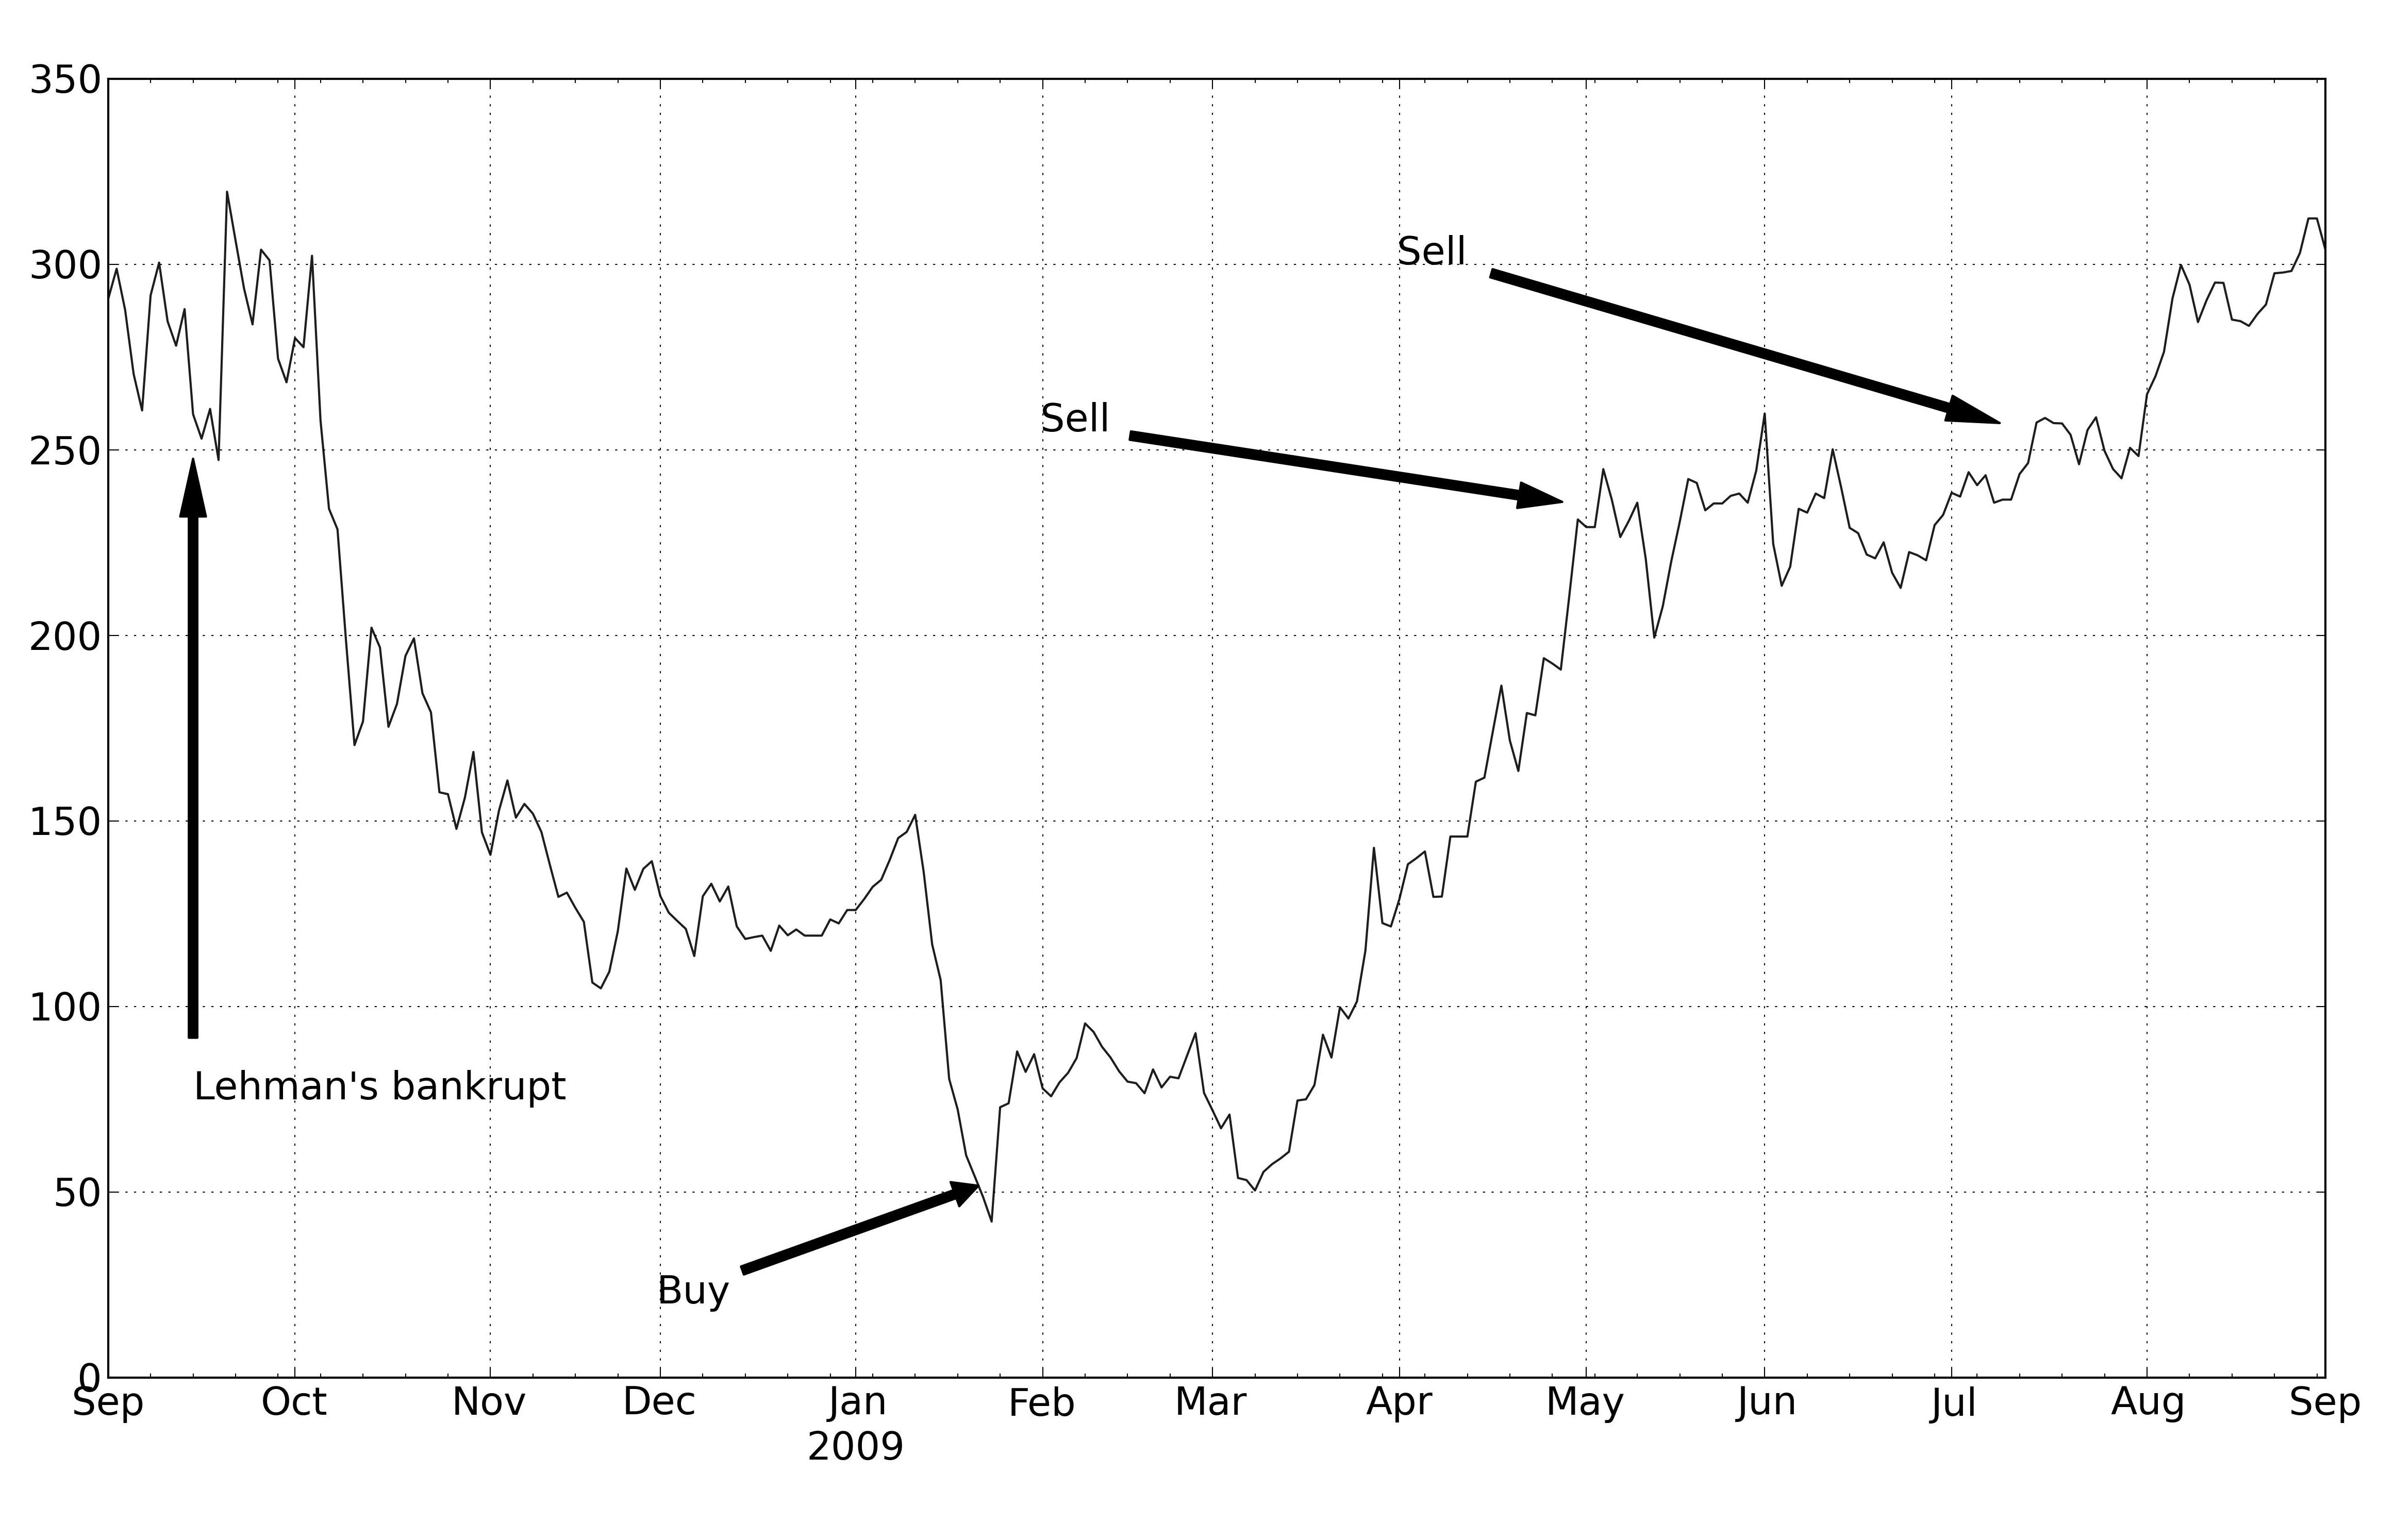
\includegraphics[width=\textwidth]{figures/raw/img-001.png} \caption{Good timing, tiny position, when trading Barclays shares in 2009. Barclays share price.\\
2009 年交易巴克莱股票时，择时很好，但仓位极小。巴克莱股价。\\
\textit{Source: Author's records.}\\
\textit{来源：作者记录。}}\end{figure}

\begin{englishblock} As figure 1 shows, that day I bought Barclays for 53p a share, and just a few months later I sold my shares for an average of \pounds 2.50 each. Although Barclays was the top performer, my other bank shares also multiplied in value. I had made a decent profit but my own panic prevented me from making much, much more. \end{englishblock}

\begin{chineseblock}如图 1 所示，那天我以每股 53 便士买入巴克莱，仅仅几个月之后，我卖出这些股票时的平均价格就达到了每股 2.50 英镑。虽然巴克莱是表现最好的那只，但我持有的其他银行股价值也都翻了倍。我确实赚到了一笔不错的利润，但正是我自己的恐慌，让我错失了本可以大得多的收益。\end{chineseblock}

\bipairgap

\begin{englishblock} I had planned carefully and meticulously, done everything right, and then at the last moment let my emotions get the better of me. \end{englishblock}

\begin{chineseblock}我原本计划周密、准备充分，前面每一步都做对了，可是在最后关头，却还是让情绪战胜了自己。\end{chineseblock}

\bilingualsection{September 2008}{2008年9月}

\begin{englishblock} Just a few months earlier I had been sitting in the same office and at the same desk. But on this particular day I had no time to think about my own money. The US government were variously trying to rescue, or had given up on, investment bank Lehman Brothers, insurer AIG, and mortgage agencies Freddie Mac and Fannie Mae. Our computer trading systems continued to run smoothly whilst the markets were in the middle of the most savage moves of a generation. But we had other things to worry about. \end{englishblock}

\begin{chineseblock}就在几个月前，我还坐在同一间办公室、同一张桌子前。但在那一天，我根本无暇顾及自己的钱。美国政府当时正在试图救助，或者已经放弃救助，投资银行雷曼兄弟、保险公司 AIG，以及按揭机构房地美和房利美。我们的计算机交易系统仍然运转平稳，而市场正处在一代人以来最剧烈的波动之中。不过，我们还有别的事情要担心。\end{chineseblock}

\bipairgap

\begin{englishblock} Although we were profitable could we trust the banks and brokers with whom we had deposited our cash? What if our clients redeemed their investments to cover holes elsewhere in their portfolio --- could we pay them? What if the whole global financial system completely seized up? We were terrified. Perhaps we should just liquidate everything, put our money into gold bars, and wait for the storm to pass. At the very least we considered reducing the risk our computers wanted to take, perhaps by half. One of our main competitors had already done exactly that. \end{englishblock}

\begin{chineseblock}虽然我们是盈利的，但我们还能信任那些替我们保管现金的银行和经纪商吗？如果客户为了填补自己其他投资组合上的窟窿而赎回资金，我们还能兑付吗？如果整个全球金融体系彻底冻结了怎么办？我们当时恐惧极了。也许我们应该把一切头寸都平掉，把钱换成金条，然后等风暴过去。至少，我们认真考虑过把计算机系统想承担的风险降下来，比如减半。我们的一个主要竞争对手已经这么做了。\end{chineseblock}

\bipairgap

\begin{englishblock} After yet another crisis meeting, where we decided to take no action for now, I left the meeting room and returned to my desk. As I sat down a colleague came over and started typing on my keyboard. \end{englishblock}

\begin{chineseblock}又开完一次危机会议之后，我们决定暂时按兵不动。我离开会议室，回到自己的座位前。刚坐下，一位同事走过来，开始在我的键盘上敲字。\end{chineseblock}

\bipairgap

\begin{englishblock} ``You'll definitely want to see this,'' he said. He pressed return, and a live estimate of today's profitability appeared on my screen. For the first time in our firm's history it showed a ten digit number. We had made over a billion dollars in a single day. Our computer system had stuck to its preprogrammed set of trading rules and mechanically exploited the market moves almost to perfection, whilst terrified humans had discussed closing it down. \end{englishblock}

\begin{chineseblock}“你肯定想看看这个。”他说。他按下回车键，我的屏幕上立刻出现了当天盈利的实时估算数字。那是我们公司历史上第一次看到一个十位数的收益数字。我们在一天之内赚了超过十亿美元。我们的计算机系统忠实执行着预先编好的那套交易规则，几乎完美地机械利用了市场波动；而与此同时，惊恐的人类却在讨论要不要把它关掉。\end{chineseblock}

\bipairgap

\begin{englishblock} Humans are better than computers at complex intellectual tasks. But as these two stories show, our emotions prevent us from fully utilising this intelligence. The solution is to use systems to make trading decisions. \end{englishblock}

\begin{chineseblock}在人类面对复杂智力任务时，通常比计算机更强。但正如这两个故事所展示的那样，我们的情绪会妨碍我们把这种智能充分发挥出来。解决办法就是用系统来做交易决策。\end{chineseblock}

\bilingualsection{Why you should start system trading now}{为什么你现在就该开始系统化交易}

\begin{englishblock} Many people have been using systems to trade in one form or another for decades, but they are still a small minority. Although there are several relatively large systematic hedge funds, including the fund I used to work for, significantly less than 10\% of actively managed global assets is fully systematically traded. But the investment world is changing and now is a better time than ever before to consider trading or investing with systems. \end{englishblock}

\begin{chineseblock}几十年来，很多人一直以这样或那样的形式使用系统进行交易，但他们仍然只是少数派。尽管市场上已经存在几家规模相当大的系统化对冲基金，包括我曾经工作过的那家，但在全球主动管理资产中，真正完全采用系统化交易的比例仍远低于 10\%。不过，投资世界正在发生变化，现在是考虑用系统进行交易或投资的最好时机。\end{chineseblock}

\bipairgap

\begin{englishblock} Firstly, institutional investors like pension funds have moved away from expensive active management, including hedge funds, to cheaper passive management. With passive management there is no ``skill'' to pay for, less trading and so lower costs. In a low inflation environment active management fees of 1\% or more are an intolerable drag on performance, even without the extra 20\% of performance charged by hedge funds. \end{englishblock}

\begin{chineseblock}首先，像养老基金这样的机构投资者，已经从昂贵的主动管理，包括对冲基金，逐步转向成本更低的被动管理。在被动管理中，没有所谓的“技能”溢价需要支付，交易更少，因此成本也更低。在低通胀环境下，哪怕只是 1\% 甚至更高的主动管理费，都会对业绩形成难以容忍的拖累，更不用说对冲基金通常还要额外收取 20\% 的业绩分成。\end{chineseblock}

\bipairgap

\begin{englishblock} Passive indexing, buying shares or bonds in fixed weights, is effectively a form of systematic trading, albeit a very simple one. I'll show how this concept can be extended and improved in the asset allocating investor example. \end{englishblock}

\begin{chineseblock}被动指数化，也就是按固定权重买入股票或债券，本质上就是一种系统化交易，只不过是非常简单的一种。我会在资产配置型投资者的例子中展示，这个概念如何进一步扩展和改进。\end{chineseblock}

\bipairgap

\begin{englishblock} The returns from hedge funds can be separated into beta --- what you can get by tracking the market, alpha --- the skill the hedge fund manager has, and alternative beta. An example of alternative beta is the additional return you can get from buying stocks with low price-to-earnings (PE) ratios, and selling those with high PE ratios --- the equity value premium. \end{englishblock}

\begin{chineseblock}对冲基金的收益可以拆分为三部分：市场本身带来的收益、基金经理技能带来的收益，以及由规则化风格暴露带来的额外收益。后一类收益的一个例子，就是买入市盈率低的股票、卖出市盈率高的股票所获得的额外回报，也就是股票价值溢价。\end{chineseblock}

\bipairgap

\begin{englishblock} Alternative beta doesn't need skill, but it can't be earned just by buying and holding shares. However it can be produced by following relatively simple rules. Some collective funds have been created to allow investors to get access to alternative beta, but they are still relatively expensive. Institutions should seriously consider using systematic rule-based trading to create in-house cheap alternative beta portfolios. The staunch systems trader example shows how this can be achieved. \end{englishblock}

\begin{chineseblock}另类贝塔并不需要特殊技能，但也不是靠简单的买入并持有股票就能得到的。不过，它可以通过遵循相对简单的规则来获得。市场上已经出现了一些集合基金，让投资者可以接触到另类贝塔，但它们的费用仍然比较高。机构投资者应当认真考虑使用基于规则的系统化交易，在内部构建低成本的另类贝塔投资组合。坚定的系统化交易者这一例子会说明具体怎么做。\end{chineseblock}

\bipairgap

\begin{englishblock} It's also easier than ever for amateurs to invest in a systematic way. Technology has revolutionised the financial industry. In the past amateur investors had to rely on yesterday's newspapers for share prices and news. Now it's possible to download historical price data for free from numerous websites. \end{englishblock}

\begin{chineseblock}如今，普通投资者也比以往任何时候都更容易用系统化方式进行投资。技术已经彻底改变了金融行业。过去，业余投资者只能依赖前一天的报纸来获取股价和新闻；而现在，你可以从大量网站上免费下载历史价格数据。\end{chineseblock}

\bipairgap

\begin{englishblock} Computing power has continued to fall in price and you can run quite sophisticated strategies on \$30 Raspberry Pi micro computers. Instead of using expensive full service stockbrokers to place trades, cheap retail brokers allow you to trade at commission levels which are a fraction of what was possible 20 years ago. \end{englishblock}

\begin{chineseblock}计算能力的价格持续下降，如今你甚至可以在一台 30 美元的 Raspberry Pi 微型计算机上运行相当复杂的策略。你也不再需要依赖昂贵的全服务股票经纪商来下单；低成本零售经纪商提供的佣金水平，仅仅是 20 年前所能达到成本的一小部分。\end{chineseblock}

\bipairgap

\begin{englishblock} There has been an explosion in the availability of numerous retail passive funds. In particular a vast array of dirt cheap exchange traded funds has appeared, allowing the passive tracking of almost every conceivable financial index. It's much easier to buy and sell securities covering a wider variety of asset classes and countries than in the past. \end{englishblock}

\begin{chineseblock}零售被动基金的供给出现了爆发式增长。尤其是，大量极其便宜的交易所交易基金开始出现，使得几乎所有可以想到的金融指数都能够被动跟踪。与过去相比，如今买卖覆盖更多资产类别、更多国家的证券都变得容易得多。\end{chineseblock}

\bipairgap

\begin{englishblock} But there have been other developments that are a mixed blessing. Derivatives like contracts for difference and spread bets allow amateurs and professionals to use leverage more easily. But unless you are careful these can quickly send your account value to zero, or even below. In the semi-automatic trader example I show how discretionary traders can trade in a relatively safe and controlled way by using a systematic framework to manage their risk. \end{englishblock}

\begin{chineseblock}不过，也有一些发展可谓利弊参半。像差价合约和点差投注这样的衍生品，使普通投资者和专业人士都能更轻松地使用杠杆。但如果你不够谨慎，它们也可能很快把你的账户净值打到零，甚至跌到负数。在半自动交易者的例子中，我会展示主观交易者如何利用系统化框架来管理风险，从而以相对安全、可控的方式进行交易。\end{chineseblock}

\bipairgap

\begin{englishblock} The offering of retail stockbrokers has been radically improved. They give you access to websites and apps that make trading as easy as ordering from Amazon. You can find brokers that allow you to submit orders automatically from software, making fully automated trading a possibility. A more recent development is the appearance of online platforms which allow you to easily implement automated strategies.\footnote{I'm less keen on the appearance of ``social trading'' websites where you ``follow'' someone else's trading strategy. It makes no sense to let an unregulated, unqualified and probably inexperienced stranger manage your money; with minimal, statistically insignificant, evidence that they are capable of doing so. \par 我对那些让你“跟随”别人交易策略的“社交交易”网站并不太认同。让一个未经监管、没有资质、而且很可能缺乏经验的陌生人来管理你的钱，是毫无道理的；更何况他们所谓有能力做到这一点的证据，往往少得可怜，而且在统计上根本没有显著性。}\end{englishblock}

\begin{chineseblock}零售股票经纪商提供的服务也已经有了巨大提升。他们给你提供网站和 App，让交易变得像在亚马逊下单一样简单。你还可以找到允许软件自动提交订单的经纪商，从而让全自动交易成为可能。近些年更进一步的发展，是出现了一批在线平台，可以让你更轻松地实现自动化策略。\end{chineseblock}

\bipairgap

\begin{englishblock} These are great tools, but they are offered solely to encourage more buying and selling. You should never forget that your broker makes more money when you trade frequently, whilst you lose out unless the extra trades are sufficiently profitable. I'll show in this book how costly overtrading is, and how you to avoid it. \end{englishblock}

\begin{chineseblock}这些工具确实很强大，但它们被提供出来，根本目的就是鼓励你更频繁地买卖。你绝不应忘记，经纪商会在你频繁交易时赚得更多；而对你来说，除非这些额外交易足够赚钱，否则你就是吃亏的一方。我会在本书中说明，过度交易的代价有多高，以及你该如何避免它。\end{chineseblock}

\bipairgap

\begin{englishblock} There are now many back-testing software packages available. These allow you to test potential strategies to see which made the most hypothetical money in the past. As I will explain in later chapters if you're not careful this will often lead to losing actual money in the present. \end{englishblock}

\begin{chineseblock}现在市面上也有许多回测软件包可供使用。它们让你能够测试潜在策略，看看哪一种在过去“理论上”赚的钱最多。但正如我会在后文解释的那样，如果你不够谨慎，这往往会让你在现实中亏掉真金白银。\end{chineseblock}

\bipairgap

\begin{englishblock} Finally, there are many books and websites containing trading systems, advice and guidance for trading, of which more in a moment. So there is no shortage of tools and advice to begin investing systematically, although you do need to be careful as they are lethal if not used safely. \end{englishblock}

\begin{chineseblock}最后，市面上还有很多书籍和网站提供交易系统、建议和指导，稍后我会详细谈到这一点。所以，开始系统化投资并不缺乏工具和建议，但你确实需要非常小心，因为如果使用不当，这些东西会非常致命。\end{chineseblock}

\bilingualsection{It's dangerous out there}{外面的世界很危险}

\begin{englishblock} Imagine for a moment you have just walked into a car dealership. Whilst admiring the vehicle on display you are approached by a slick suited salesman. \end{englishblock}

\begin{chineseblock}想象一下，你刚走进一家汽车经销店。正当你欣赏展厅里的汽车时，一位穿着体面的销售人员走了过来。\end{chineseblock}

\begin{quote}
\begingroup\color{\englishbodycolorname} ``This looks great, but it's a bit small for me. What other models do you have?'' you ask. ``Actually this is the only model we make,'' he replies. ``Okay... Would you recommend the convertible, or is the fuel consumption too high?'' ``We don't have a convertible.'' ``Right. How much extra would it cost to get alloy wheels and air conditioning?'' ``Nothing. We don't do them.'' ``Does it come in red?'' ``No. Just black.'' \endgroup
\end{quote}

\begin{quote}
\begingroup\color{\chinesebodycolorname}“这车看起来不错，不过对我来说有点小。你们还有别的车型吗？”你问。“其实我们只生产这一款。”他回答。“好吧……那敞篷版怎么样？还是说油耗太高？”“我们没有敞篷版。”“明白了。如果加装合金轮毂和空调，要多花多少钱？”“不用加钱。因为我们根本不提供这些配置。”“那有红色的吗？”“没有，只有黑色。”\endgroup
\end{quote}

\begin{englishblock} You'd be pretty surprised. In reality a new car buyer is offered so many options that the possible permutations usually run into millions! Car dealers can do this because cars are modular --- made up of individual components which can be easily changed. When buying a new car we can specify different engines or add options like a fancy stereo. Later on we can still change certain parts like the tyres. \end{englishblock}

\begin{chineseblock}你大概会非常吃惊。现实中，买新车的人通常会面对多得惊人的可选配置，各种排列组合往往多达数百万种。汽车经销商之所以能这么做，是因为汽车是模块化产品--- 由许多可以轻松更换的独立部件组成。买新车时，我们可以指定不同的发动机，或者添加高级音响之类的配置。即便买了之后，像轮胎这样的部分也还能继续更换。\end{chineseblock}

\bipairgap

\begin{englishblock} Now consider the large number of books and websites describing various trading systems. Many are too vague to be considered systematic but others include quite detailed rules. Nearly all of these publicly available trading systems are not modular, and can't be easily adapted. You don't have the opportunity to ask the author questions like: \end{englishblock}

\begin{chineseblock}现在再看看那些介绍各种交易系统的大量书籍和网站。其中很多内容过于模糊，根本算不上系统化；另一些则给出了相当详细的规则。但几乎所有公开可见的交易系统都不是模块化的，也无法轻松调整。你没法向作者提出下面这样的问题：\end{chineseblock}

\begin{quote}
\begingroup\color{\englishbodycolorname} ``I notice you used a 20-day moving average here. When would it make sense to use a 30-day moving average? You say we should put 2.5\% of our capital into each trade. Why? What will happen if I put 5\% in? I like your trading rules, but how would I use those in my own position management framework? How can I use this to trade gasoline futures?'' \endgroup
\end{quote}

\begin{quote}
\begingroup\color{\chinesebodycolorname}“我注意到你这里用了 20 日移动平均线。那么在什么情况下用 30 日移动平均线会更合适？你说每笔交易应该投入 2.5\% 的资金，为什么？如果我投入 5\% 会怎样？我喜欢你的交易规则，但我该如何把它们放进我自己的仓位管理框架中？我又该怎样用这套方法去交易汽油期货？”\endgroup
\end{quote}

\begin{englishblock} I will answer these questions, and many more, later in the book. Now let's return to the imaginary conversation with our hypothetical car dealer. \end{englishblock}

\begin{chineseblock}这些问题，以及更多类似的问题，我都会在本书后面逐一回答。现在，让我们回到刚才那段与假想汽车销售员的对话。\end{chineseblock}

\begin{quote}
\begingroup\color{\englishbodycolorname} ``How fast does it go?'' ``It does exactly 150.6 miles an hour.'' ``Wow! I bet it drinks fuel at that speed. What's the fuel economy like at 55?'' ``No you weren't listening. It always does precisely 150.6. No faster or slower.'' ``Isn't that a little... dangerous?'' ``Well it was fine on the manufacturer's test track.'' \endgroup
\end{quote}

\begin{quote}
\begingroup\color{\chinesebodycolorname}“它能跑多快？”“时速正好 150.6 英里。”“哇！那这个速度下油耗一定很夸张吧。那如果时速 55 英里时，油耗怎么样？”“不，你没听明白。它永远都精确地跑 150.6。不会更快，也不会更慢。”“这是不是有点……危险？”“嗯，在厂家测试跑道上它表现挺好的。”\endgroup
\end{quote}

\begin{englishblock} Once again consider the many publicly available trading systems. Many advocate trading extremely quickly, holding positions for only a few days, minutes or even seconds. In many markets traded by amateur investors that will lead to extremely high trading costs. Frighteningly the majority of trading systems also suggest holding sizable positions which are far too risky unless you know in advance you will be a brilliant trader who is also very lucky. Using these systems is like driving at 200mph and hoping you won't crash or run out of fuel. \end{englishblock}

\begin{chineseblock}再回头看看那些公开可得的交易系统。很多系统都主张极快地交易，持仓时间可能只有几天、几分钟，甚至几秒钟。在许多由普通投资者参与的市场里，这会带来极其高昂的交易成本。更可怕的是，大多数交易系统还建议持有相当大的仓位，而这通常风险高得离谱，除非你事先就知道自己会是一位天才交易者，同时还会特别走运。使用这类系统，就像以每小时 200 英里的速度开车，同时祈祷自己既不会撞车，也不会耗尽燃料。\end{chineseblock}

\bipairgap

\begin{englishblock} To take an example, one expert on spread betting proposes putting at most 10\%, but usually 5\%, of your capital into each trade. Sensibly he suggests you diversify, holding several positions in different markets at once. He then proposes using a particular type of trading rule which means positions would be held on average for about a week.\footnote{This is a real system, but I will not identify the author. It is by no means the worst system I have seen. \par 这是一套真实存在的系统，但我不会点名作者。它绝不是我见过最糟糕的系统。}\end{englishblock}

\begin{chineseblock}举个例子，一位点差投注专家建议你每笔交易最多投入 10\% 的资金，而通常是 5\%。他也明智地建议你进行分散化，同时在不同市场持有多个头寸。然后，他又建议使用一种特定类型的交易规则，这意味着平均每笔仓位会持有大约一周。\end{chineseblock}

\bipairgap

\begin{englishblock} This sounds safe, but should actually come with a significant health warning. To overcome the trading costs this would generate on an index spread bet and break even you would need to make a return of 83\% a year.\footnote{If you are interested I explain why on page 192. \par 如果你感兴趣，我会在第 192 页解释原因。} Worse still, to avoid a high chance of losing most of your entire investment you'd need to average 256\% a year after costs; implying an annualised pre-cost return of 339\%!\footnote{The calculation for this is on page 151. \par 这一计算见第 151 页。}\end{englishblock}

\begin{chineseblock}这听起来似乎很安全，但实际上理应附带醒目的风险警告。要覆盖这种做法在指数点差投注上产生的交易成本，并做到盈亏平衡，你每年需要获得 83\% 的回报。更糟的是，为了避免有很高概率亏掉你大部分本金，你在扣除成本后每年平均需要赚到 256\%；这意味着年化的成本前收益必须达到 339\%！ \end{chineseblock}

\bipairgap

\begin{englishblock} Thinking that you can overcome these odds is a sign of serious overconfidence, the main weakness of all traders and investors. I will explain why these systems are dangerous, and how to make your trading safer. \end{englishblock}

\begin{chineseblock}认为自己能够战胜这样的胜算，本身就是严重过度自信的表现，而这恰恰是所有交易者和投资者最大的弱点。我会解释为什么这些系统很危险，以及如何让你的交易变得更安全。\end{chineseblock}

\bilingualsection{Why you should read this book}{为什么你应该读这本书}

\begin{englishblock} I don't believe there is any magic system that will automatically make you huge profits, and you should be wary of anyone who says otherwise, especially if they want to sell it to you. Instead success in systematic trading is mostly down to avoiding common mistakes such as over complicating your system, being too optimistic about likely returns, taking excessive risks, and trading too often. I will help you avoid these errors. This won't guarantee vast returns, but it will make failure less likely. \end{englishblock}

\begin{chineseblock}我并不相信存在什么魔法系统，能够自动为你赚取巨额利润。对于任何这么说的人，你都应该保持警惕，尤其是在他们还想把这套系统卖给你的时候。相反，系统化交易的成功，更多取决于你能否避开一些常见错误，例如把系统搞得过于复杂、对可能的收益过于乐观、承担过度风险，以及交易过于频繁。我会帮助你避开这些错误。这样做并不能保证你暴富，但会让失败的概率更低。\end{chineseblock}

\bipairgap

\begin{englishblock} My main aim isn't just to give you a single predefined system for trading, but to provide you with a modular framework which can be adapted to meet your needs. Part three describes the framework in detail. Just like you can choose different engines and tyres on a car, my framework includes options for different trading rules and position sizing calculations. \end{englishblock}

\begin{chineseblock}我的主要目标，不只是给你一套预先定义好的单一交易系统，而是提供一个可以根据你的需求加以调整的模块化框架。第三部分会详细讲解这个框架。就像你可以买车时选择不同的发动机和轮胎一样，我的框架也包含多种交易规则和仓位规模计算方法可供选择。\end{chineseblock}

\bipairgap

\begin{englishblock} I haven't just pulled a bunch of components out of a parts bin. Each element of the framework has been carefully designed with months of careful research, built on many years of experience. I'll explain the available options, which I prefer, and why. \end{englishblock}

\begin{chineseblock}我并不是随手从零件箱里抓出一堆组件拼在一起。这个框架中的每一个元素，都是在多年经验的基础上，经过数月细致研究后精心设计出来的。我会解释有哪些可选项、我个人偏好哪些，以及原因是什么。\end{chineseblock}

\bipairgap

\begin{englishblock} Just like cars can be modified I will show you how to incorporate your own trading rules and change other parts of the framework. I will warn you of the dangers of being too aggressive, which will result in your bank account blowing up like an over-tuned engine. I'll discuss the correct amount to bet on a particular trade, and how long to hold positions for. \end{englishblock}

\begin{chineseblock}就像汽车可以改装一样，我会告诉你如何把自己的交易规则纳入这个框架，以及如何修改框架中的其他部分。我也会提醒你，过于激进有多危险；那会让你的账户像调校过头的发动机一样直接炸掉。我还会讨论，一笔具体交易到底该下多大的注，以及仓位应该持有多久。\end{chineseblock}

\bipairgap

\begin{englishblock} In part four I show how to create trading strategies for each of the three example groups I mentioned in the preface. Sticking with the car analogy you can create a sturdy family car for asset allocating investing, an experimental kit car for semi-automatic trading, or a sporty two seater convertible of a trading system if you are a staunch systems trader. But before you get your fingers greasy you need to do some preparation. So the first part of the book which follows is all about theory, and in the second part I explain how to use your tools safely. \end{englishblock}

\begin{chineseblock}在第四部分中，我会展示如何针对我在前言里提到的三类示例人群，分别构建交易策略。继续沿用汽车的比喻，你可以为资产配置型投资打造一辆结实耐用的家用车，为半自动交易打造一辆实验性的套件车，而如果你是一位坚定的系统化交易者，那么你完全可以造出一辆跑车式的双座敞篷交易系统。不过，在真正动手之前，你还需要先做好准备。因此，接下来的第一部分讲的是理论，第二部分则会解释如何安全地使用你的工具。\end{chineseblock}
